\chapter{MixVRTの実装}\label{cha:Implementation}
本章では、試作した\toolName の実装について説明する。
% なお、本研究で用いる、\toolName の各処理部が取得または生成する画像名を、以下に定義する。
% \begin{itemize}
%     \item Webページの変更前画像
%     \item Webページの変更後画像
%     \item 高解像度にしたWebページの変更前画像
%     \item 高解像度にしたWebページの変更後画像
%     \item 画像比較に基づく削除箇所を赤枠で囲むことで強調表示した、Webページの変更前画像
%     \item 画像比較に基づく追加箇所を緑枠で囲むことで強調表示した、Webページの変更後画像
%     \item HTMLコードにおけるbody要素内の追加とstyle要素内の追加のどちらか、
%           または両方の追加による影響を受けた箇所を赤枠で囲むことで強調表示した、Webページの変更前画像
%     \item HTMLコードにおけるbody要素内の削除とstyle要素内の削除のどちらか、
%           または両方の削除による影響を受けた箇所を緑枠で囲むことで強調表示した、Webページの変更後画像
%     \item HTMLコードの変更に基づく影響箇所を色付きの枠で囲むことで強調表示した、Webページの変更前画像
%     \item HTMLコードの変更に基づく影響箇所を色付きの枠で囲むことで強調表示した、Webページの変更後画像
%     \item レイアウトの不具合箇所を色付きの枠で囲むことで強調表示した、Webページの変更前画像
%     \item レイアウトの不具合箇所を色付きの枠で囲むことで強調表示した、Webページの変更後画像
% \end{itemize}
\par
\toolName のシステム構成を、図\ref{fig:System}に示す。
\begin{figure}[tp]
    \begin{center}
        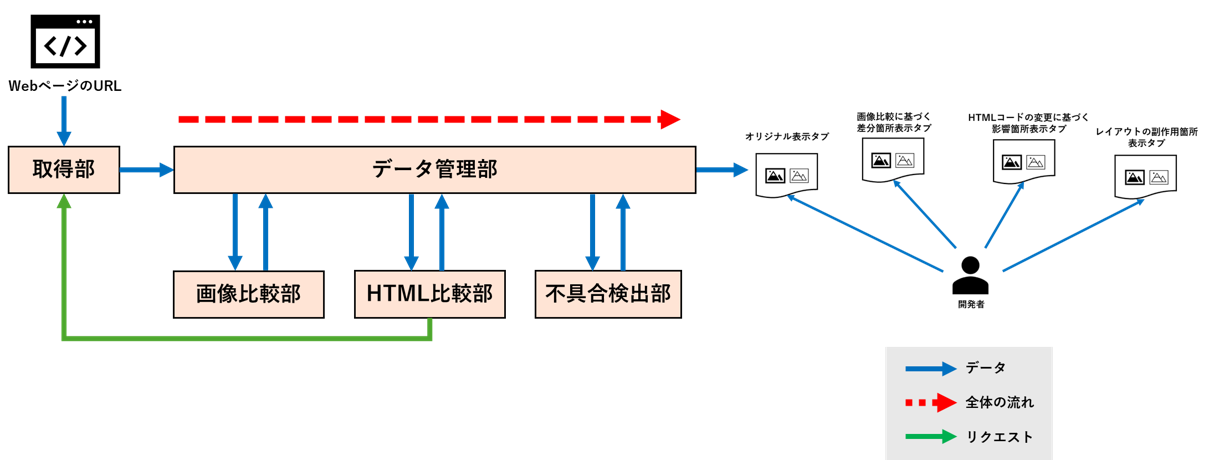
\includegraphics[width=1.0\columnwidth]{image/4_System_4.png}
        \caption{\toolName のシステム構成}
        \label{fig:System}
    \end{center}
\end{figure}
% 私の開発したツールは、まずユーザーがWebページのURLを入力します。
% このURLを受け取ると、ツールは該当するWebページから画像を取得し、
% これらの画像に対して特定の処理を行います。処理された画像は"static/images"ディレクトリに保存されます。
% そして、Flaskがローカルサーバを提供し、
% "templates"フォルダにあるHTMLコードが"static/images"ディレクトリを参照できるようになっています。
% この仕組みにより、ユーザーはローカルに立てられたFlaskサーバを通じて、
% Webページ上で生成された画像を確認することができます。
\toolName は、以下の6つの処理部から構成する。
\begin{itemize}
    \item データ管理部
    \item 取得部
    \item 画像比較部
    \item HTML比較部
    \item 不具合検出部
          % \item 表示部
          % \item 表示部
\end{itemize}
% \begin{itemize}
%     \item 取得部
%     \item 画像比較部
%           \begin{enumerate}
%               \item 差分箇所検出
%           \end{enumerate}
%     \item HTML比較部
%           \begin{enumerate}
%               \item 差分コード生成
%               \item 差分コード解析
%               \item 影響箇所強調HTMLコード生成
%           \end{enumerate}
%     \item レイアウト副作用箇所抽出部
%     \item 表示部
% \end{itemize}
以降、\toolName を構成する6つの処理部について説明する。
\par

\section{データ管理部}\label{sec:data_admin_section}
データ管理部は、システム内の各処理部間における、データの伝達を担い、他の処理部とのデータのやり取りとデータの保存を行う。
なお、本論文におけるデータとは、処理前後のWebページの画像やHTMLコードであり、
やり取りしたデータはデータ管理部が持つディレクトリに保存する。
また、取得部(\ref{sec:Web_data_get_section}節で後述)のみ、データ管理部とのデータのやり取りが一方向である(図\ref{fig:System}を参照)。
% また、取得部(\ref{sec:Web_data_get_section}節で後述)と表示部(\ref{sec:Interface_Display_Section}節で後述)のみ、データ管理部とのデータのやり取りが一方向である(図\ref{fig:System}を参照)。
% また、取得部とデータ管理部の間におけるデータのやり取りは、取得部からデータ管理部への一方向のみであり、
% データ管理部と表示部の間におけるデータのやり取りは、データ管理部から表示部への一方向のみである。
\par
データ管理部における最初のデータのやり取りは、取得部である。
取得部からデータを受け取ると、そのデータをデータ管理部のbase\_dirディレクトリに保存する。
保存した後、データがそれ以外に存在しない場合、
% Flaskを用いて構築したローカルサーバ上で動作するWebページ(
\toolName による視覚的回帰テスト結果を閲覧できるWebページ(\ref{sec:Flask}節を参照)に、
Webページの変更前画像のみを出力し、全体の処理を終了する。
データがそれ以外に存在する場合、
画像比較部(\ref{sec:Difference_extraction_section}節で後述)、HTML比較部(\ref{sec:Affected_area_extraction}節で後述)、不具合検出部(\ref{sec:Layout_bug_extraction_section}節で後述)の順に
データのやり取りを行う。
各処理部とのやり取りを終えると、
データ管理部は、\toolName による視覚的回帰テスト結果を閲覧できるWebページに、
\ref{subsec:MixVRT_IO}節で述べた8つのPNG形式の画像を出力し、全体の処理を終了する。
% なお、出力先のWebページは、\toolName による視覚的回帰テストで生成した画像の確認が効率的に行えるWebページを開発者に提供する。
\par
各処理部との間でやり取りしたデータを保存する各ディレクトリを、以下に示す。
\begin{itemize}
    \item base\_dirディレクトリ:\\
          取得部で取得したWebページの画像とHTMLコードを保存する。
          %   \begin{itemize}
          %       \item currentディレクトリ:\\
          %             Webページの変更前画像と変更前HTMLコードを保存する。
          %       \item latestディレクトリ:\\
          %             Webページの変更後画像と変更後HTMLコードを保存する。
          %   \end{itemize}
    \item diff\_dirディレクトリ:\\
          画像比較部、HTML比較部、不具合検出部でやり取りしたデータを保存する。
          % \item disp\_dirディレクトリ:\\
          %       表示部に出力するデータを保存する。
          % Webページの変更前画像と変更後画像、Webページの変更前HTMLコードと変更後HTMLコードを用いて、
\end{itemize}
また、各ディレクトリに保存するデータの詳細を、以下の表\ref{tb: base_dir_data}と表\ref{tb: diff_dir_data}に示す。
\begin{table}[tp]
    \caption{base\_dirディレクトリに保存するデータの詳細}
    \label{tb: base_dir_data}
    \centering
    \begin{tabular}{c|l}
        \hline
        データ                      & \multicolumn{1}{c}{説明}                          \\
        \hline \hline
        Webページの変更前画像       & \toolName の初回実行時に取得する画像。            \\ \hline
        Webページの変更前HTMLコード & \toolName の初回実行時に取得するHTMLコード。      \\ \hline
        Webページの変更後画像       & \toolName の2回目以降実行時に取得する画像。       \\ \hline
        Webページの変更後HTMLコード & \toolName の2回目以降実行時に取得するHTMLコード。 \\ \hline
    \end{tabular}
\end{table}

\begin{table}[tp]
    \caption{diff\_dirディレクトリに保存するデータの詳細}
    \label{tb: diff_dir_data}
    \centering
    \begin{tabular}{c|l}
        \hline
        データ                     & \multicolumn{1}{c}{説明}                                       \\
        \hline \hline
        変更前高解像度画像         & Webページの変更前画像を高解像度にした画像。                    \\ \hline
        変更後高解像度画像         & Webページの変更後画像を高解像度にした画像。                    \\ \hline
        変更前高解像度二値化画像   & 変更前高解像度画像を二値化した画像。                           \\ \hline
        変更後高解像度二値化画像   & 変更後高解像度画像を二値化した画像。                           \\ \hline
        削除箇所二値化画像         & 変更前高解像度二値化画像から共通部分を削除した画像。           \\ \hline
        追加箇所二値化画像         & 変更後高解像度二値化画像から共通部分を削除した画像。           \\ \hline
        削除箇所強調二値化画像     & 削除箇所二値化画像の白い部分を強調した画像。                   \\ \hline
        追加箇所強調二値化画像     & 追加箇所二値化画像の白い部分を強調した画像。                   \\ \hline
        差分箇所赤枠強調マスク画像 & 削除箇所強調二値化画像の白い部分を囲む赤枠のみを抽出した画像。 \\ \hline
        差分箇所緑枠強調マスク画像 & 追加箇所強調二値化画像の白い部分を囲む緑枠のみを抽出した画像。 \\ \hline    
        % \begin{tabular}{l}差分箇所赤枠強調画像\\\end{tabular}  & \begin{tabular}{l}画像比較に基づく差分箇所を、\\色付きの枠で囲むことで強調表示した、Webページの変更前画像。\end{tabular}                                      \\ \hline
        % \begin{tabular}{l}差分箇所緑枠強調画像\\\end{tabular}  & \begin{tabular}{l}画像比較に基づく差分箇所を、\\色付きの枠で囲むことで強調表示した、Webページの変更後画像。\end{tabular}                                      \\ \hline
        % \begin{tabular}{l}影響箇所赤枠強調画像\\\end{tabular}  & \begin{tabular}{l}画像比較に基づく差分箇所を、\\色付きの枠で囲むことで強調表示した、Webページの変更前画像。\end{tabular}                                     \\ \hline
        % \begin{tabular}{l}影響箇所緑枠強調画像\\\end{tabular} & \begin{tabular}{l}画像比較に基づく差分箇所を、\\色付きの枠で囲むことで強調表示した、Webページの変更後画像。\end{tabular}                                     \\ \hline
        影響箇所赤枠強調マスク画像 & 枠付き変更前画像から赤枠のみを抽出した画像。                   \\ \hline
        影響箇所緑枠強調マスク画像 & 枠付き変更後画像から緑枠のみを抽出した画像。                   \\ \hline
    \end{tabular}
\end{table}

% \toolName を2回実行した際の、データ管理部と各処理部とのやり取りを行ったデータを保存するディレクトリの構造を、以下に示す。

% % directory

% \begin{lstlisting}[language=, basicstyle=\ttfamily]
% .
% ├── base_dir/
% │   ├── (2回目実行時のタイムスタンプ)/
% │   │   ├── html/
% │   │   │   └── html_(2回目実行時のタイムスタンプ).html
% │   │   └── img/
% │   │       └── img_(2回目実行時のタイムスタンプ).png
% │   ├── current/ 
% │   │   ├── html/
% │   │   │   └── html_(1回目実行時のタイムスタンプ).html
% │   │   └── img/
% │   │       └── img_(1回目実行時のタイムスタンプ).png
% │   ├── initial/
% │   │   ├── html/
% │   │   │   └── html_(1回目実行時のタイムスタンプ).html
% │   │   └── img/
% │   │       └── img_(1回目実行時のタイムスタンプ).png
% │   └── latest/
% │       ├── html/
% │       │   └── html_(2回目実行時のタイムスタンプ).html
% │       └── img/
% │           └── img_(2回目実行時のタイムスタンプ).png
% └── diff_dir/
%      ├── diff_img_png/
%      │   ├── diff_af_img.png
%      │   └── diff_bf_img.png
%      ├── diff_rec_html_high_png/
%      │   ├── diff_rec_af_html.png
%      │   └── diff_rec_bf_html.png
%      ├── diff_rec_img_high_png/
%      │   ├── diff_rec_af_img.png
%      │   └── diff_rec_bf_img.png
%      ├── diff_html_txt/
%      │   └── diff_html.txt
%      ├── modified_html/
%      │   └── templates/
%      │       ├── modified_testPage_af.html
%      │       └── modified_testPage_bf.html
%      ├── modified_html_png/
%      │   ├── modified_testPage_af.png
%      │   └── modified_testPage_bf.png
%      ├── modifiled_html_high_png/
%      │   ├── modified_testPage_af_high.png
%      │   └── modified_testPage_bf_high.png
%      ├── original_high_png/
%      │   ├── img_af_high.png
%      │   └── img_bf_high.png
%      └── sub_effect_png/
%          ├── subEffect_af.png
%          └── subEffect_bf.png
% \end{lstlisting}

% \begin{itemize}
%     \item 取得部からデータ管理部
%     \item データ管理部から表示部
% \end{itemize}

% 5つの各処理部から受け付けるデータを、以下に示す。
% \begin{itemize}
%     \item 取得部:
%           \begin{itemize}
%               \item Webページの変更前画像と変更後画像
%           \end{itemize}
%     \item 画像比較部:
%           \begin{itemize}
%               \item 画像比較に基づく差分箇所を色付きの枠で囲むことで強調表示した、Webページの変更前画像と変更後画像
%               \item 上記の画像を高解像度にし、枠のみを抽出した、削除強調マスク画像と追加強調マスク画像
%           \end{itemize}
%     \item HTML比較部:
%           \begin{itemize}
%               \item HTMLコードの変更に基づく影響箇所を色付きの枠で囲むことで強調表示した、Webページの変更前画像と変更後画像
%               \item 上記の画像を高解像度にし、枠のみを抽出した、削除強調マスク画像と追加強調マスク画像
%           \end{itemize}
%     \item 副作用抽出部:
%           \begin{itemize}
%               \item レイアウトの副作用箇所を色付きの枠で囲むことで強調表示した、Webページの変更前画像と変更後画像
%           \end{itemize}
%     \item 不具合抽出部:
%           \begin{itemize}
%               \item レイアウトの不具合箇所を色付きの枠で囲むことで強調表示した、Webページの変更前画像と変更後画像
%           \end{itemize}
% \end{itemize}

% なお、\toolName の初回実行時は、取得部からWebページの画像とHTMLを受け取ると、\toolName 全体の処理を終了する。

\section{取得部}\label{sec:Web_data_get_section}
取得部は、テキスト端末上からWebページのURLを入力として受け取り、URLから取得したWebページの画像とHTMLコードを、データ管理部のbase\_dirディレクトリに出力する。
なお、HTML比較部から取得部に、枠付きWebページのURL(\ref{sec:Flask}節を参照)を与えて呼び出す場合があり(図\ref{fig:System}と\ref{sec:Affected_area_extraction}節を参照)、
その場合は、取得したデータをデータ管理部のdiff\_dirディレクトリに出力する。
\par
Webページの画像取得には、Selenium WebDriver(\ref{sec:Selenium_WebDriver}節を参照)を用いて、WebページのURLからWebページの画像を取得する。
なお、取得するWebページの画像は、フルページのスクリーンショット画像である。
WebページのHTMLコード取得には、Pythonライブラリの1つであるrequests(\ref{sec:requests}節を参照)を用いて、
WebページのURLからWebページのHTMLコードを取得する。

\section{画像比較部}\label{sec:Difference_extraction_section}
画像比較部は、データ管理部のbase\_dirディレクトリからWebページの変更前画像と変更後画像を受け取り、
画像比較に基づく差分箇所を色付きの枠で囲むことで強調表示した、Webページの変更前画像と変更後画像を生成する。
また、それらの画像から枠のみを残してそれ以外の部分を黒くすることで、差分箇所を囲む色付きの枠のみを抽出した、「差分箇所赤枠強調マスク画像」と「差分箇所緑枠強調マスク画像」も生成する。
生成した画像は、データ管理部のbase\_dirディレクトリに出力する。
\par
画像比較部の処理の流れを、以下に示す。
\begin{enumerate}
    \item 高解像度画像生成処理
    \item 適応的二値化処理
    \item 差分検出処理
    \item 膨張処理
    \item 輪郭検出処理
    \item 枠描画処理
\end{enumerate}
また、\toolName のテスト対象とするWebページの変更前画像と変更後画像の例を、図\ref{fig: img_original_bf_af}に示す。
\begin{figure}[tp]
    \begin{center}
        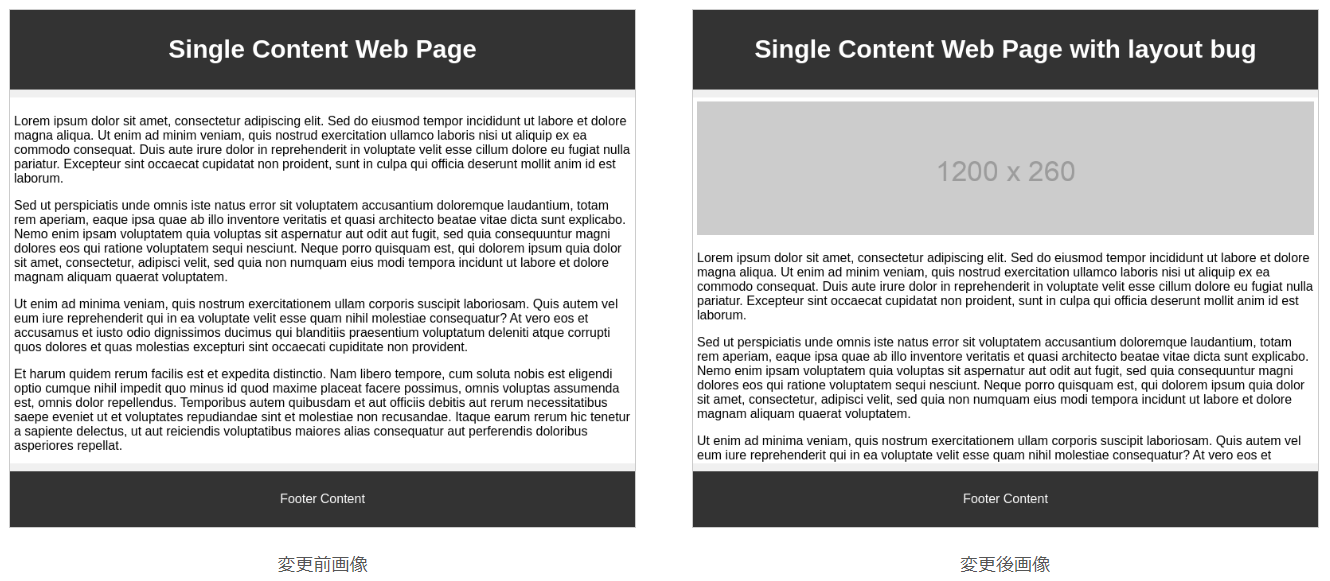
\includegraphics[width=1.0\columnwidth]{image/4_img_original_bf_af.png}
        \caption{\toolName のテスト対象とするWebページの変更前画像と変更後画像の例}
        \label{fig: img_original_bf_af}
    \end{center}
\end{figure}
以降、具体例に図\ref{fig: img_original_bf_af}を用いて、画像比較部の各処理について説明する。

\subsection{高解像度画像生成処理}\label{subsec:Generate_high_images}
高解像度画像生成処理は、図\ref{fig: img_original_bf_af}のWebページの変更前画像と変更後画像をそれぞれ高解像度画像にした、「変更前高解像度画像」と「変更後高解像度画像」を生成する。
「変更前高解像度画像」と「変更後高解像度画像」を、図\ref{fig: img_high_original_bf_af}に示す。
\begin{figure}[tp]
    \begin{center}
        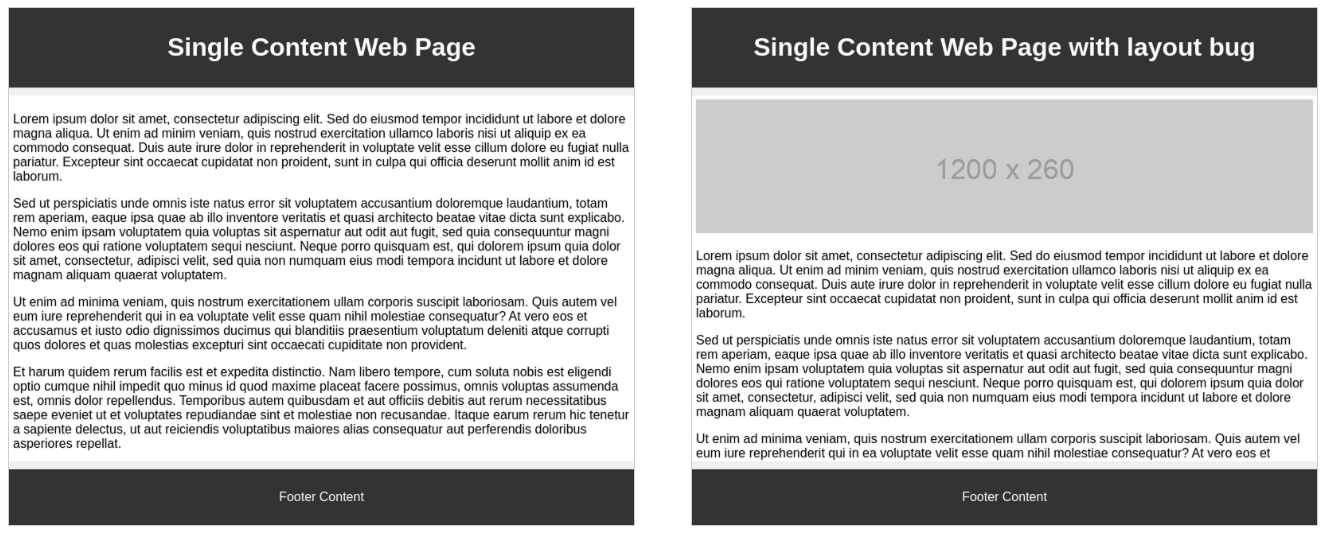
\includegraphics[width=1.0\columnwidth]{image/4_img_high_original_bf_af.png}
        \caption{「変更前高解像度画像」と「変更後高解像度画像」}
        \label{fig: img_high_original_bf_af}
    \end{center}
\end{figure}
この処理は、輪郭検出処理(\ref{subsec:contour_detection_processing}節で後述)の精度を向上するために必要である。
なお、生成した高解像度画像は他の処理部で使用するため、「変更前高解像度画像」と「変更後高解像度画像」をデータ管理部のbase\_dirディレクトリに出力する。
\par
高解像度画像を生成する流れを、以下に示す。なお、リサイズに使用するリサンプリングフィルタには、LANCZOSフィルタ(\ref{sec:pillow}節を参照)を用いる。
\begin{enumerate}
    \item PillowのImage.open関数(\ref{sec:pillow}節を参照)を用いて、Webページの画像パスから画像を読み込む。
    \item 画像の幅と高さを取得する。
    \item 画像の拡大率を設定する。本研究では、$2$とする。
    \item 画像のサイズ変更時に使用するリサンプリングフィルタを設定する。本研究では、PillowのImage.LANCZOSフィルタ(\ref{sec:pillow}節を参照)を用いる。
    \item Webページの画像を、画像の幅と高さにそれぞれ画像の拡大率を掛けたサイズの高解像度画像にリサイズする。
\end{enumerate}


\subsection{適応的二値化処理}\label{subsec:Adaptive_Binarisation}
適応的二値化処理は、図\ref{fig: img_high_original_bf_af}の「変更前高解像度画像」と「変更後高解像度画像」のそれぞれに対して、適応的二値化を行う。
この処理により、画像の一部が明るく、他の部分が暗い場合においても、全体として均一な二値化画像を生成できるため、
輪郭検出処理(\ref{subsec:contour_detection_processing}節で後述)の精度向上につながる。
処理の結果として、適応的二値化処理を行った、「変更前高解像度二値化画像」と「変更後高解像度二値化画像」を生成する。
「変更前高解像度二値化画像」と「変更後高解像度二値化画像」を、図\ref{fig: img_high_bin_bf_af}に示す。
\begin{figure}[tp]
    \begin{center}
        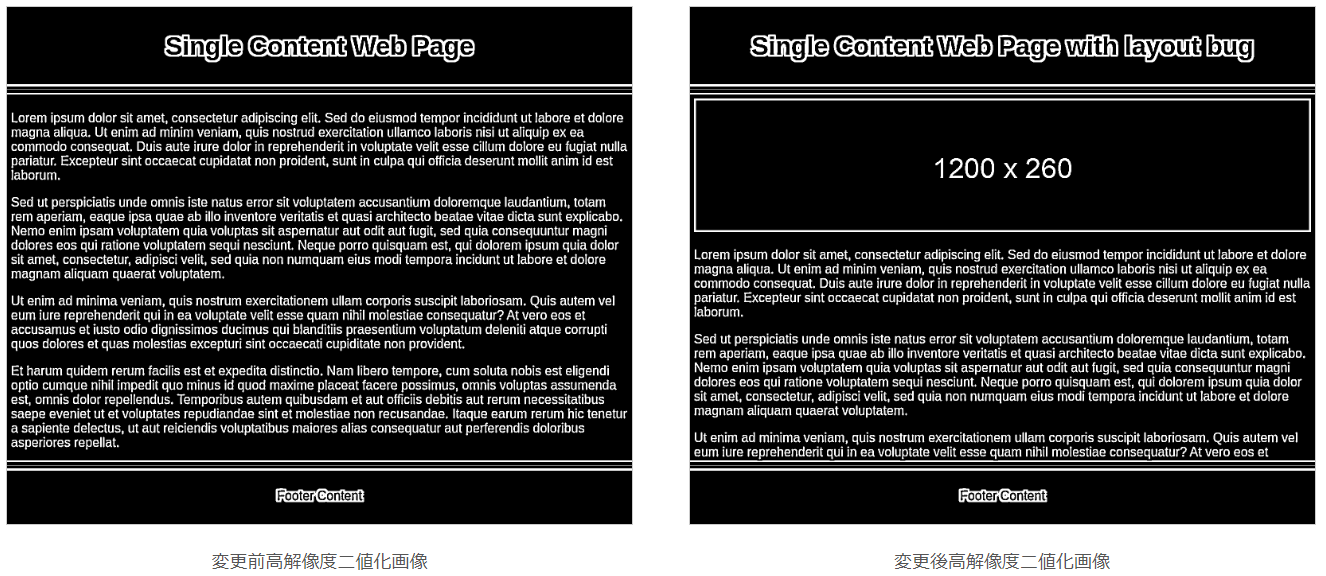
\includegraphics[width=1.0\columnwidth]{image/4_img_high_bin_bf_af.png}
        \caption{「変更前高解像度二値化画像」と「変更後高解像度二値化画像」}
        \label{fig: img_high_bin_bf_af}
    \end{center}
\end{figure}
\par
「変更前高解像度画像」と「変更後高解像度画像」に対して、それぞれ適応的二値化を行う流れを、以下に示す。
\begin{enumerate}
    \item OpenCVのimread関数(\ref{sec:opencv}節を参照)を用いて、画像を読み込む。
    \item OpenCVのcvtColor関数(\ref{sec:opencv}節を参照)を用いて、画像をグレースケール化する。
    \item OpenCVのadaptiveThreshold関数(\ref{sec:opencv}節を参照)を用いて、グレースケール画像に対して白黒反転を伴う適用的二値化を行う。
\end{enumerate}

\subsection{差分検出処理}\label{subsec:difference_detection_process}
差分検出処理は、図\ref{fig: img_high_bin_bf_af}の「変更前高解像度二値化画像」と「変更後高解像度二値化画像」に対して、差分検出を行う。
処理の結果として、Webページの変更前画像から削除された箇所と、Webページの変更後画像に追加された箇所をそれぞれ白い部分として可視化した、
「削除箇所二値化画像」と「追加箇所二値化画像」を生成する。
「削除箇所二値化画像」と「追加箇所二値化画像」を、図\ref{fig: img_del_add_bin_bf_af}に示す。
\begin{figure}[tp]
    \begin{center}
        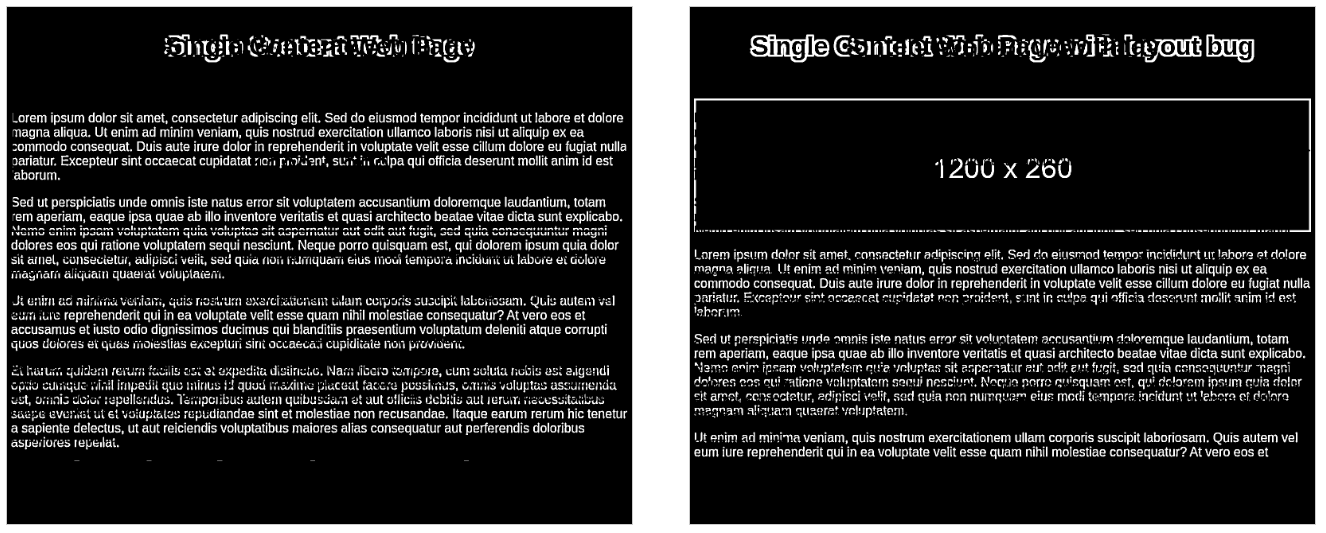
\includegraphics[width=1.0\columnwidth]{image/4_img_del_add_bin_bf_af.png}
        \caption{「削除箇所二値化画像」と「追加箇所二値化画像」}
        \label{fig: img_del_add_bin_bf_af}
    \end{center}
\end{figure}
図\ref{fig: img_del_add_bin_bf_af}を見ると、
図\ref{fig: img_high_bin_bf_af}の「変更前高解像度二値化画像」と「変更後高解像度二値化画像」を重ねたときの共通部分である白い箇所が消えており、
「変更前高解像度二値化画像」には、削除箇所が残り、「変更後高解像度二値化画像」には、追加箇所が残る。
これにより、輪郭検出処理(\ref{subsec:contour_detection_processing}節で後述)で、削除箇所を赤枠で、追加箇所を緑枠で囲むことができる。
\par
「変更前高解像度二値化画像」と「変更後高解像度二値化画像」に対して、差分検出処理を行う流れを、以下に示す。
\begin{enumerate}
    \item OpenCVのsubtract関数(\ref{sec:opencv}節を参照)の第一引数に「変更前高解像度二値化画像」を指定し、
          第二引数に「変更後高解像度二値化画像」を指定する。
    \item 1のsubtract関数によって、変更前の画像には存在するが変更後の画像には存在しない箇所を可視化した「削除箇所二値化画像」を生成する。
    \item subtract関数(\ref{sec:opencv}節を参照)の第一引数に「変更後高解像度二値化画像」を指定し、
          第二引数に「変更前高解像度二値化画像」を指定する。
    \item 3のsubtract関数によって、変更後の画像には存在するが変更前の画像には存在しない箇所を可視化した「追加箇所二値化画像」を生成する。
\end{enumerate}

\subsection{膨張処理}\label{subsec:dilation}
% (\ref{sec:dilation}節を参照)
膨張処理は、「削除箇所二値化画像」と「追加箇所二値化画像」のそれぞれの白い部分の形状とサイズを強調する。
この処理により、削除箇所と追加箇所の輪郭検出処理(\ref{subsec:contour_detection_processing}節で後述)を高める。
処理の結果として、膨張処理を行った、「削除箇所強調二値化画像」と「追加箇所強調二値化画像」を生成する。
「削除箇所強調二値化画像」と「追加箇所強調二値化画像」を、図\ref{fig: img_del_add_highlight_bin}に示す。
\begin{figure}[tp]
    \begin{center}
        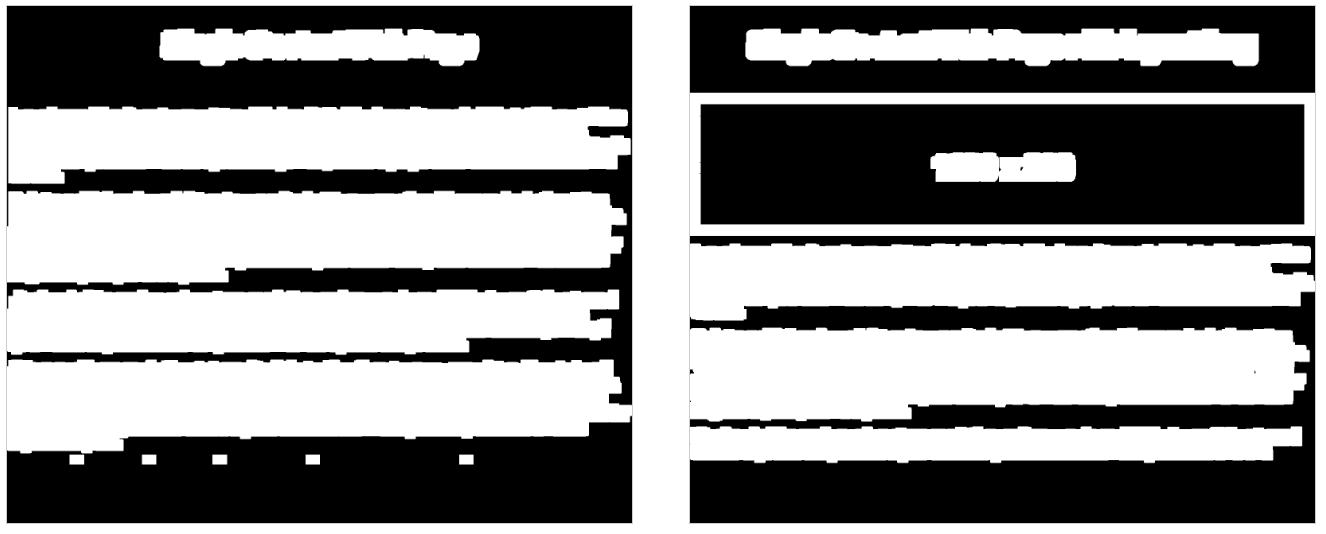
\includegraphics[width=1.0\columnwidth]{image/4_img_del_add_highlight_bin.png}
        \caption{「削除箇所強調二値化画像」と「追加箇所強調二値化画像」}
        \label{fig: img_del_add_highlight_bin}
    \end{center}
\end{figure}
\par
「削除箇所二値化画像」と「追加箇所二値化画像」に対して、膨張処理を適用する流れを、以下に示す。
\begin{enumerate}
    \item 特定の形状とサイズを持つカーネルを設定する。本研究では、5x5ピクセルの正方形カーネルを採用する。
    \item 設定したカーネルを用いて、膨張処理を適用する。適用後、画像内の削除箇所または追加箇所が拡大する。
    \item 2の膨張処理を複数回適用する。本研究では、膨張処理を6回繰り返すことで削除箇所または追加箇所を強調する。
    \item 膨張処理によって生成した「削除箇所強調二値化画像」と「追加箇所強調二値化画像」を輪郭検出処理に渡す。
\end{enumerate}

\subsection{輪郭検出処理}\label{subsec:contour_detection_processing}
輪郭検出処理は、OpenCVのfindContours関数(\ref{sec:opencv}節を参照)を用いて、図\ref{fig: img_del_add_highlight_bin}の「削除箇所強調二値化画像」と「追加箇所強調二値化画像」に対して、
削除箇所の輪郭と追加箇所の輪郭をそれぞれ検出する。
この処理の結果として、削除箇所の輪郭リストと追加箇所の輪郭リストを取得する。

\subsection{枠描画処理}\label{subsec:Bounding box drawing process}
枠描画処理は、Webページの変更前画像と変更後画像に対して、
輪郭検出処理(\ref{subsec:contour_detection_processing}節を参照)で取得した輪郭リストを用いて、
図\ref{fig: img_diff_highlight}に示した、
画像比較に基づく差分箇所を、色付きの枠で囲むことで強調表示した、Webページの変更前画像と変更後画像を生成する。
\begin{figure}[tp]
    \begin{center}
        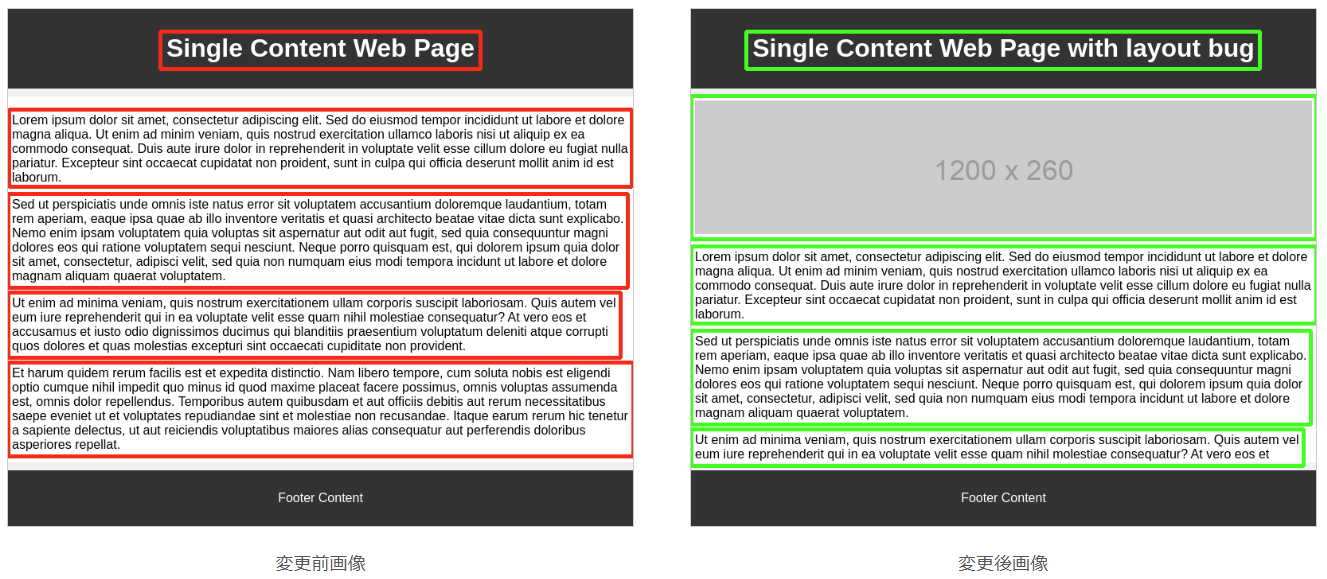
\includegraphics[width=1.0\columnwidth]{image/4_img_diff_highlight.png}
        \caption{画像比較に基づく差分箇所を、色付きの枠で囲むことで強調表示した、Webページの変更前画像と変更後画像}
        \label{fig: img_diff_highlight}
    \end{center}
\end{figure}
また、それらの画像から枠のみを残してそれ以外の部分を黒くすることで、差分箇所を囲む色付きの枠のみを抽出した、
「差分箇所赤枠強調マスク画像」と「差分箇所緑枠強調マスク画像」を生成する。
「差分箇所赤枠強調マスク画像」と「差分箇所緑枠強調マスク画像」を、図\ref{fig: img_diff_highlight_mask}に示す。
\begin{figure}[tp]
    \begin{center}
        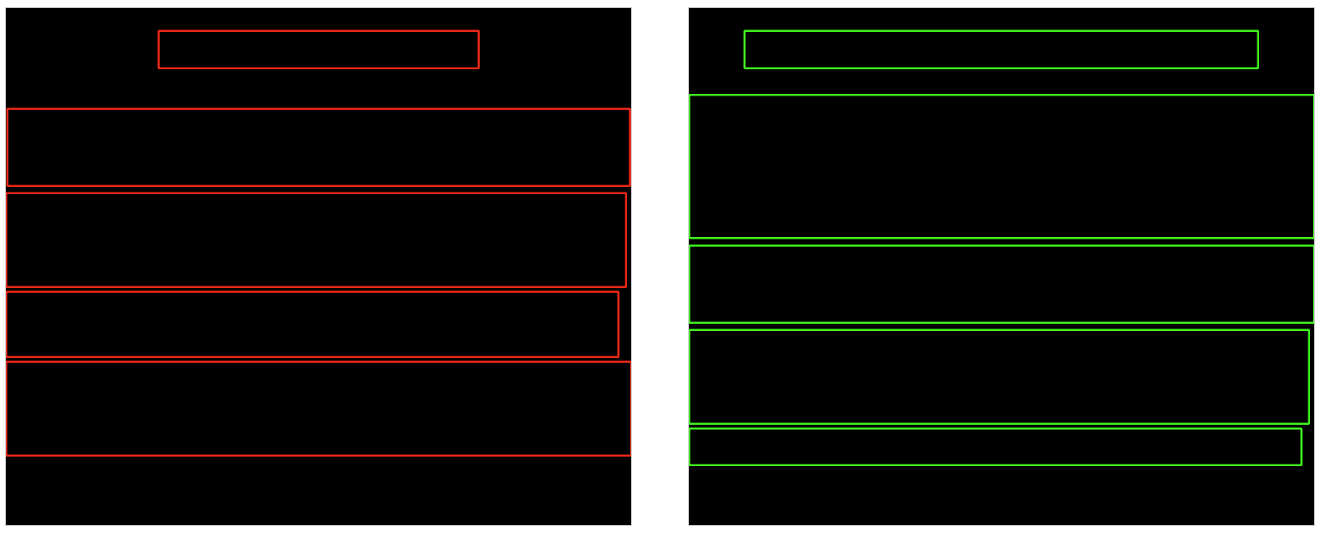
\includegraphics[width=1.0\columnwidth]{image/4_img_diff_highlight_mask.png}
        \caption{「差分箇所赤枠強調マスク画像」と「差分箇所緑枠強調マスク画像」}
        \label{fig: img_diff_highlight_mask}
    \end{center}
\end{figure}
\par
枠描画処理の流れを、以下に示す。
\begin{enumerate}
    \item boundingRect関数(\ref{sec:opencv}節を参照)を用いて、輪郭リストの各要素である輪郭データから、輪郭を囲む矩形の座標と幅、高さを取得する。
    \item 取得した矩形情報を引数に指定したrectangle関数(\ref{sec:opencv}節を参照)を用いて、Webページの変更前画像上に赤枠、Webページの変更後画像上に緑枠を描画する。
    \item np.zeros関数(\ref{sec:numpy}節を参照)を用いて、Webページの変更前画像と変更後画像のそれぞれと同じサイズの黒画像を生成する。
    \item 取得した矩形情報を引数に指定したrectangle関数を用いて、生成した2つの黒画像に対して、一方の黒画像には赤枠を、もう一方の黒画像には緑枠を描画する。
\end{enumerate}


%%%% HTML比較 %%%%
% 画像比較部は、データ管理部のbase\_dirディレクトリからWebページの変更前画像と変更後画像を受け取り、
% 画像比較に基づく差分箇所を色付きの枠で囲むことで強調表示したWebページの変更前画像と変更後画像を生成する。
% また、それらの画像から枠のみを残してそれ以外の部分を黒くすることで、差分箇所を囲む色付きの枠のみを抽出した、「差分箇所赤枠強調マスク画像」と「差分箇所緑枠強調マスク画像」も生成する。
% 生成した画像は、データ管理部のbase\_dirディレクトリに出力する。
% \par
% 画像比較部の処理の流れを、以下に示す。
% \begin{enumerate}
%     \item 高解像度画像生成処理
%     \item 適応的二値化処理
%     \item 差分検出処理
%     \item 膨張処理
%     \item 輪郭検出処理
%     \item 枠描画処理
% \end{enumerate}
% また、\toolName のテスト対象とするWebページの変更前画像と変更後画像の例を、図\ref{fig: img_original_bf_af}に示す。
% \begin{figure}[tp]
%     \begin{center}
%         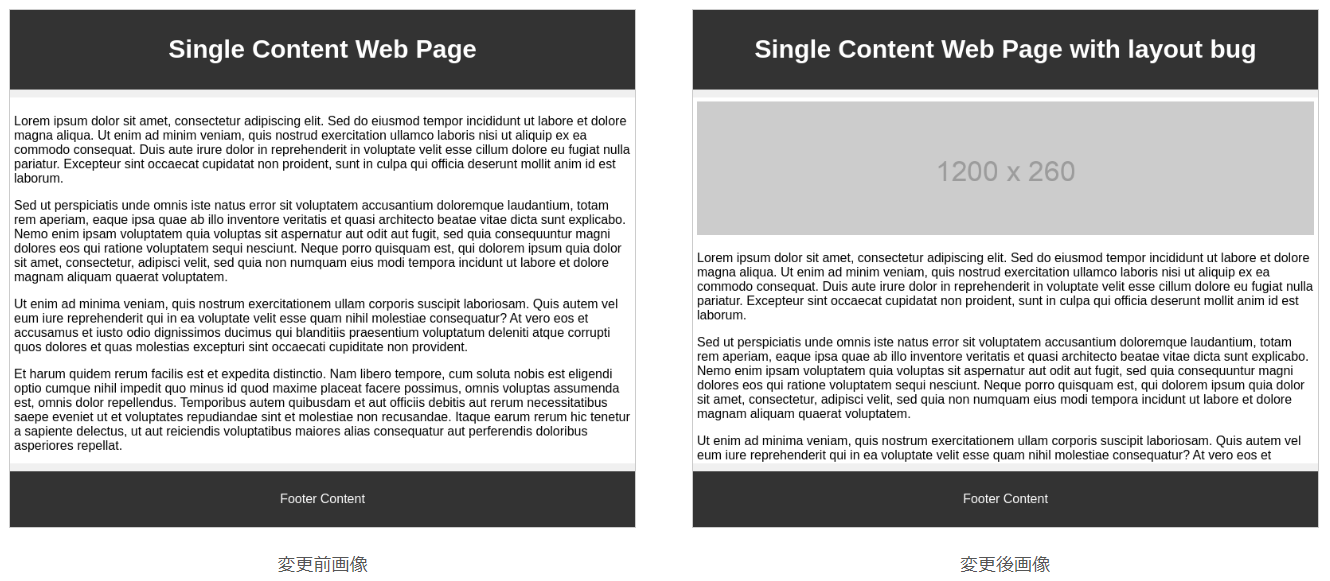
\includegraphics[width=1.0\columnwidth]{image/4_img_original_bf_af.png}
%         \caption{\toolName のテスト対象とするWebページの変更前画像と変更後画像の例}
%         \label{fig: img_original_bf_af}
%     \end{center}
% \end{figure}
% 以降、具体例に図\ref{fig: img_original_bf_af}を用いて、画像比較部の各処理について説明する。
\section{HTML比較部}\label{sec:Affected_area_extraction}
HTML比較部は、データ管理部のbase\_dirディレクトリからWebページの変更前HTMLコードと変更後HTMLコードを受け取り、
HTMLコードの変更に基づく影響箇所を色付きの枠で囲むことで強調表示した、Webページの変更前画像と変更後画像を生成する。
また、それらの画像から枠のみを残してそれ以外の部分を黒くすることで、影響箇所を囲む色付きの枠のみを抽出した、「影響箇所赤枠強調マスク画像」と「影響箇所緑枠強調マスク画像」も生成する。
生成した画像は、データ管理部のdiff\_dirディレクトリに出力する。
\par
HTML比較部の処理の流れを、以下に示す。
\begin{enumerate}
    \item 差分コード生成処理
    \item 枠付きHTMLコード生成処理
    \item 枠抽出処理
\end{enumerate}
以降、図\ref{fig: img_original_bf_af}の例で挙げたWebページの、変更前HTMLコードと変更後HTMLコードを具体例に、
HTML比較部の各処理について説明する。

\subsection{差分コード生成処理}\label{subsec:diff_file_generate}
差分コード生成処理は、Webページの変更前HTMLコードと変更後HTMLコードを行ごとに比較して、txt形式の差分コードを生成する。
生成したtxt形式の差分コードの例を、ソースコード\ref{lst:diff_html}に示す。
ソースコード\ref{lst:diff_html}の3行目を見ると、先頭に"-"が付いており、この行は削除行であることを示す。
また、ソースコード\ref{lst:diff_html}の4行目および8行目を見ると、先頭に"+"が付いており、この行は追加行であることを示す。
このように、生成したtxt形式の差分コードには、コードの追加行の先頭に"+"、削除行の先頭に"-"を付加する。
\begin{figure}[tp]
    \begin{lstlisting}[language=HTML, caption=生成したtxt形式の差分コードの例, label=lst:diff_html]
<body>
    <header>
-         <h1>Single Content Web Page</h1>
+         <h1>Single Content Web Page with layout bug</h1>
    </header>
    <div class="container">
        <div class="main-content">
+             <img src="https://via.placeholder.com/1200x260" alt="Placeholder Image">
              // テキスト文省略
        </div>
    </div>
    <footer>
        <p>Footer Content</p>
    </footer>
</body>
    \end{lstlisting}
\end{figure}
\par
差分コードを生成する処理を、以下に示す。
\begin{enumerate}
    \item 変更前HTMLコードと変更後HTMLコードをそれぞれHTMLデータとして読み込む。
    \item HTMLデータ内の$<$p$>$タグ内のテキスト内に存在する余分な空白や改行を取り除く(\ref{sec:text_change}節を参照)ために、以下を行う。
          \begin{enumerate}
              \item 変更前と変更後のHTMLデータを解析するためのBeautifulSoupオブジェクト(\ref{sec:beautifulsoup}節を参照)をそれぞれ初期化する。
              \item BeautifulSoupオブジェクトに対して、find\_all関数(\ref{sec:beautifulsoup}節を参照)を用い、HTMLデータ内の全ての$<$p$>$タグを格納したリストを生成する。
              \item get\_text関数(\ref{sec:beautifulsoup}節を参照)を用いて、生成したリストの各要素内における$<$p$>$タグのテキストを取得する。
              \item Pythonの文字列関数であるsplit関数を用いて、取得した各テキストを空白文字で分割する。
              \item Pythonの文字列関数であるjoin関数を用いて、分割したテキストを再び空白文字で連結する。
              \item BeautifulSoupオブジェクトをstring型に変換し、HTMLデータ形式に戻す。
          \end{enumerate}
    \item difflib(\ref{sec:difflib}節を参照)のDifferクラスとcompare関数を用いて、2つのHTMLデータ間を行ごとに比較し、差分コードを生成する。
    \item 生成した差分コードから、行の先頭が"?"から始まる行を除外する。
    \item 差分コードをtxt形式で保存する。
\end{enumerate}

% \subsection{差分コード解析処理}\label{subsec:diff_file_analyze}
% 差分コード解析処理は、差分コード生成処理から差分コードを受け取り、差分コードからbody要素内の変更箇所とstyle要素内の変更箇所を検出する。
% \par
% 差分コードを解析する処理を、以下に示す。

% 枠付きHTMLコード生成するためには、以下の処理を行う。
% body要素内の変更箇所を検出する。
% 差分コードの先頭の行に対して、以下の処理を行う。
% 1.body要素外であるか判定する。body要素外ならば、以下の処理を行う。
% 1. 先頭行が"-"であれば、
% body要素内の各先頭行に"+"または"-"がある箇所を探す。
% "+"や"-"であれば、その行に対して以下の操作を行う。
% 1."+"または"-"を削除する。
% 2.行にimgタグが含まれている場合、img用の枠を囲むCSSクラスを追加する。
% 3.行にimgタグが含まれていない場合、行中に開始タグが存在するかを確認する。
% 4.行中に開始タグが存在する場合は、タグ内にclass属性が既にあるかどうか確認する。行中に開始タグが存在しない場合は、何もしない。
% 5.class属性があれば、class=""の中の末尾に枠をつけるクラスを追加する。
% 6.class属性が無ければ、終了タグ直前に枠をつけるクラスを追加する。

% body要素内の変更箇所に枠をつけるCSSクラスを追加する。
% style要素内の変更箇所を検出する。
% style要素内の変更箇所に枠をつけるCSSクラスを追加する。

\subsection{枠付きHTMLコード生成処理}\label{subsec:modified_html_generate}
枠付きHTMLコード生成処理は、差分コード生成処理から差分コードを受け取り、枠付き変更前HTMLコードと枠付き変更後HTMLコードを生成する。
なお、枠付き変更前HTMLコードは、影響箇所(\ref{cha:Function}を参照)における削除箇所に赤枠をつけるCSSクラス(\ref{subsubsec: css_define}節を参照)を付加した、変更前HTMLコードと定義する。
また、枠付き変更後HTMLコードは、影響箇所における追加箇所に緑枠をつけるCSSクラスを付加した、変更後HTMLコードと定義する。
生成したHTMLコードは、データ管理部のdiff\_dirディレクトリに出力する。
\par
差分コードから、枠付き変更前HTMLコードと枠付き変更後HTMLコードを生成する処理を、以下に示す。
\begin{enumerate}
    \item body要素解析処理
    \item CSSセレクタ抽出処理
    \item CSSクラス付加処理
\end{enumerate}

\subsubsection{body要素解析処理}\label{subsubsec: body_analysis}
body要素解析処理は、差分コード生成処理から受け取った差分コードにおいて、body要素内で変更があったタグ要素のstyle属性にCSSクラス\cite{CssSelector}を付加し、
未完成の枠付き変更前HTMLコードを格納したリストmodified\_before\_linesと、未完成の枠付き変更後HTMLコードを格納したリストmodified\_after\_linesを生成する。
\par
body要素解析処理の流れを、以下に示す。
なお、modified\_before\_linesとmodified\_after\_linesを、それぞれ空リストとして初期化する。
また、現在処理中の行において、削除行であると判定する変数flag\_beforeの値と、追加行であると判定する変数flag\_afterの値を、それぞれFalseで初期化する。
さらに、差分コードの全ての行に対して、先頭行から順に1行ずつ、以下の処理を行う。
\begin{enumerate}
    \item 行がbody要素外の場合:
          \begin{enumerate}
              \item 行の先頭が"-"の場合、modified\_before\_linesに行を追加する。
              \item 行の先頭が"+"の場合、modified\_after\_linesに行を追加する。
              \item 行の先頭がそれ以外の場合、modified\_before\_linesとmodified\_after\_linesの両方に行を追加する。
          \end{enumerate}
    \item 行がbody要素内の場合:
          \begin{enumerate}
              \item 行の先頭が"-"または"+"の場合:
                    \begin{enumerate}
                        \item 行の先頭が"-"の場合、flag\_beforeの値をTrueにし、"-"を取り除く
                        \item 行の先頭が"+"の場合、flag\_afterの値をTrueにし、"+"を取り除く
                        \item 行中に"\textless img"を含む場合:
                              \begin{enumerate}
                                  \item imgタグ用のCSSクラスを付加したdivタグでimgタグを囲む。
                              \end{enumerate}
                        \item 行中に"\textless img"を含まない場合:
                              \begin{enumerate}
                                  \item 行中に"class="を含む場合、開始タグのstyle属性にbody要素用のCSSクラスを付加する。
                                  \item 行中に"class="を含まない場合、開始タグの終了記号直前にbody要素用のCSSクラスを付加する。
                              \end{enumerate}
                    \end{enumerate}
              \item 行の先頭がそれ以外の場合:\\
                    flag\_beforeとflag\_afterの両方の値をFalseにする。
              \item flag\_beforeの値がTrue、 かつ、flag\_afterの値がFalseの場合、modified\_before\_linesに行を追加する。
              \item flag\_beforeの値がFalse、 かつ、flag\_afterの値がTrueの場合、modified\_after\_linesに行を追加する。
              \item それ以外の場合、modified\_before\_linesとmodified\_after\_linesの両方に行を追加する。
          \end{enumerate}
    \item modified\_before\_linesとmodified\_after\_linesを、CSSクラス付加処理に出力する。
\end{enumerate}

\subsubsection{CSSセレクタ抽出処理}\label{subsubsec: style_analysis}
CSSセレクタ抽出処理は、差分コード生成処理から受け取った差分コードにおいて、style要素内で変更があったCSSセレクタ\cite{CssSelector}を、差分コードから全て抽出する。
抽出したCSSセレクタは、リストにそれぞれ格納し、CSSクラス付加処理(\ref{subsubsec: css_define}節に後述)に出力する。
\par
CSSセレクタ抽出処理の流れを、以下に示す。
\begin{enumerate}
    \item 変更があったCSSセレクタを格納するリストであるchanged\_selectorsを、空リストとして初期化する。
    \item 現在処理中のCSSセレクタを保持するための変数であるcurrent\_selectorの値を、Noneに初期化する。
    \item 差分コードの全ての行に対して、先頭行から順に1行ずつ文字列の判定をし、判定結果に応じて、以下の処理を行う。
          \begin{enumerate}
              \item CSSセレクタの開始を示す"\{"を含む行を見つけた場合:
                    \begin{enumerate}
                        \item 行中のCSSセレクタのみを抽出する。
                        \item changed\_selectors内に抽出したセレクタが存在せず、かつ、行が変更を示す"+"、または、"-"で始まる場合、
                              CSSセレクタをchanged\_selectorsに格納する。
                        \item current\_selectorの値にCSSセレクタを格納し、現在処理中のCSSセレクタを更新する。
                    \end{enumerate}
              \item CSSセレクタの終了を示す"\}"を含む行を見つけた場合:
                    \begin{enumerate}
                        \item current\_selectorの値にNoneを格納し、現在処理中のCSSセレクタをリセットする。
                        \item 3に戻る。
                    \end{enumerate}
              \item current\_selectorの値にCSSセレクタが格納されており、行が変更を示す"+"、または、"-"で始まる場合:
                    \begin{enumerate}
                        \item changed\_selectors内に、current\_selectorに格納されているCSSセレクタが存在しないならば、
                              そのCSSセレクタをchanged\_selectorsに格納する。
                    \end{enumerate}
          \end{enumerate}
    \item changed\_selectorsを、CSSクラス付加処理に出力する。
\end{enumerate}

\subsubsection{CSSクラス付加処理}\label{subsubsec: css_define}
CSSクラス付加処理は、未完成の枠付き変更前HTMLコードのstyle要素の末尾に、影響箇所における削除箇所に赤枠をつけるCSSクラスを付加し、枠付き変更前HTMLコードを生成する。
また、未完成の枠付き変更後HTMLコードのstyle要素の末尾に、影響箇所における追加箇所に緑枠をつけるCSSクラスを付加し、枠付き変更後HTMLコードを生成する。
\par
影響箇所に色枠をつける6種類のCSSクラスを、以下に定義する。
\begin{itemize}
    \setlength{\itemsep}{0pt}
          \setlength{\parsep}{0pt}
    \item UNIQUE\_CLASS\_BEFORE\_CSS:\\
          body要素内での削除、または変更があった画面要素を赤枠で囲むスタイルを定義したCSSクラス。
    \item UNIQUE\_CLASS\_AFTER\_CSS:\\
          body要素内での追加、または変更があった画面要素を緑枠で囲むスタイルを定義したCSSクラス。
    \item IMAGE\_WRAPPER\_CLASS\_BEFORE\_CSS:\\
          body要素内での削除、または、CSSの変更があった画像を赤枠で囲むスタイルを定義したCSSクラス。
    \item IMAGE\_WRAPPER\_CLASS\_AFTER\_CSS:\\
          body要素内での追加、または、CSSの変更があった画像を緑枠で囲むスタイルを定義したCSSクラス。
    \item SELECTORS\_CLASS\_BEFORE\_CSS:\\
          style要素内で変更があった、CSSセレクタ群に赤枠を付加するスタイルを定義したCSSクラス。
    \item SELECTORS\_CLASS\_AFTER\_CSS:\\
          style要素内で変更があった、CSSセレクタ群に緑枠を付加するスタイルを定義したCSSクラス。
\end{itemize}
\par
CSSクラス付加処理の流れを、以下に示す。
\begin{enumerate}
    \item body要素解析処理から、未完成の枠付き変更前HTMLコードを格納したリストmodified\_before\_linesと、未完成の枠付き変更後HTMLコードを格納したリストmodified\_after\_linesを受け取る。
    \item CSSセレクタ抽出処理から、変更があったCSSセレクタを格納するリストchanged\_selectorsを受け取る。
    \item 枠付き変更前HTMLコードを格納するリストfinal\_before\_linesと、枠付き変更後HTMLコードを格納するリストfinal\_after\_linesを空リストとして初期化する。
    \item modified\_before\_lines内の先頭行から順に、各行に対して、以下の処理を行う。
          \begin{enumerate}
              \item "$<$/style$>$"を含まない行の場合、final\_before\_linesに行を追加する。
              \item "$<$/style$>$"を含む行を見つけた場合:
                    \begin{enumerate}
                        \item final\_before\_linesに、UNIQUE\_CLASS\_BEFORE\_CSSと\\IMAGE\_WRAPPER\_CLASS\_BEFORE\_CSSを追加する。
                        \item changed\_selectorsの要素数が$0$より大きい場合、final\_before\_linesに、\\SELECTORS\_CLASS\_BEFORE\_CSSを追加する。
                        \item final\_before\_linesに、"$<$/style$>$"を含む行を加える。
                    \end{enumerate}
          \end{enumerate}
    \item modified\_after\_lines内の先頭行から順に、各行に対して、以下の処理を行う。
          \begin{enumerate}
              \item "$<$/style$>$"を含まない行の場合、final\_after\_linesに行を追加する。
              \item "$<$/style$>$"を含む行を見つけた場合:
                    \begin{enumerate}
                        \item final\_after\_linesに、UNIQUE\_CLASS\_AFTER\_CSSと\\IMAGE\_WRAPPER\_CLASS\_AFTER\_CSSを追加する。
                        \item changed\_selectorsの要素数が$0$より大きい場合、final\_after\_linesに、\\SELECTORS\_CLASS\_AFTER\_CSSを追加する。
                        \item final\_after\_linesに、"$<$/style$>$"を含む行を加える。
                    \end{enumerate}
          \end{enumerate}
    \item final\_before\_lineとfinal\_after\_linesを、データ管理部のdiff\_dirディレクトリに出力する。
\end{enumerate}
% style要素内の末尾に、body要素内で変更があった、画像以外のタグ要素にCSSクラスを付加する。なお、画像の追加や削除、変更があれば、imgタグ用のCSSクラスを付加する。
% また、CSSセレクタ抽出処理から受け取った、変更があったCSSセレクタを格納するリストchanged\_selectorsに、1つ以上のCSSセレクタを含む場合は、
% CSSセレクタ用のCSSクラスをstyle要素内の末尾に付加する。

\subsection{枠抽出処理}\label{subsec:frame_extraction}
枠抽出処理は、
Webページの変更前画像と枠付きを行ったWebページの変更前画像を比較し、赤枠のみを抽出した「影響箇所赤枠強調マスク画像」を生成する。
また、Webページの変更後画像と枠付きを行ったWebページの変更後画像を比較し、緑枠のみを抽出した「影響箇所緑枠強調マスク画像」を生成する。
なお、枠付きを行った、Webページの変更前画像と変更後画像を、それぞれ「枠付き変更前画像」と「枠付き変更後画像」と定義する。
生成した画像は、データ管理部のdiff\_dirディレクトリに出力する。
\par
枠抽出処理の流れを、以下に示す。
\begin{enumerate}
    \item データ管理部のbase\_dirディレクトリから、Webページの変更前画像と変更後画像を受け取る。
    \item データ管理部のdir\_dirディレクトリから、枠付き変更前HTMLコードと枠付き変更後HTMLコードを受け取る。
    \item 枠付き変更前HTMLコードと枠付き変更後HTMLコードを、ローカルサーバ上(\ref{sec:Flask}節を参照)でそれぞれWebページとして公開する
    \item 3で公開したそれぞれのWebページのURLを、取得部に渡す。これにより、取得部は、
          枠付き変更前画像と枠付き変更後画像を取得し、取得した画像をデータ管理部のdiff\_dirディレクトリに出力する。
    \item データ管理部のdiff\_dirディレクトリから、枠付き変更前画像と枠付き変更後画像を取得する。
    \item Webページの変更前画像と枠付き変更前画像を比較し、「影響箇所赤枠強調マスク画像」を生成する
    \item Webページの変更後画像と枠付き変更後画像を比較し、「影響箇所緑枠強調マスク画像」を生成する
\end{enumerate}

% \section{影響箇所検出部}\label{sec:Affected_area_extraction}
% HTMLコードの変更に基づく影響箇所抽出部は、Webページ情報取得部で取得した変更前後のWebページのHTMLコードを用いて影響箇所を特定する。
% 概要としては、差分コードを生成し、差分コードから枠付き処理を行った変更前後のHTMLコードを生成した後、そのHTMLコードをFlaskのテンプレートエンジンを用いてWebページを表示し、Webページ情報取得部によってそのWebページの画像を取得する。
% 元のWebページ画像と枠付き処理をしたWebページ画像を比較して枠のみを抽出する。
% 具体的には、まず、Pythonライブラリの一つであるdifflibモジュールを用いて、変更前後のHTMLコードから差分コードを生成する。
% 生成した差分コードは、コードの追加行には"+", 削除行には"-", 変更前後のHTMLコードにどちらにも存在しない行には"?"が先頭に付き、"?"を除いた差分コードを解析対象とする。
% 差分コードは、bodyタグ内とstyleタグ内を対象とする。
% もし、bodyタグ内で先頭に"+"や"-"があれば、コードの追加や削除、変更があったとして、その箇所に枠付き処理を行うCSSクラスを追加し、先頭の"+"か"-"を削除する。
% styleタグ内の場合は、CSSクラスのセレクタ名のみの変更やスタイルのみの変更、またはその両方の変更があったCSSクラスを対象として、そのCSSクラスに対して枠付きを行うスタイルを適用する。
% この場合においても、解析した行の先頭に"+", "-"があれば削除する。
% 差分コードから枠付き処理を行った変更前後のHTMLコードを生成した後は、そのHTMLコードをFlaskのテンプレートエンジンを用いてWebページとして表示し、そのWebページの画像を取得する。
% そして、元のWebページ画像と枠付き処理をしたWebページ画像を比較して枠のみを抽出する。
\section{不具合検出部}\label{sec:Layout_bug_extraction_section}
不具合検出部は、データ管理部のdiff\_dirディレクトリから「差分箇所赤枠強調マスク画像」と「差分箇所緑枠強調マスク画像」、「影響箇所赤枠強調マスク画像」と「影響箇所緑枠強調マスク画像」、
「Webページの変更前画像」と「Webページの変更後画像」を受け取り、
レイアウトの不具合箇所を、色付きの枠で囲むことで強調表示した、Webページの変更前画像と変更後画像を生成する。
なお、レイアウトの不具合箇所を、赤枠で囲むことで強調表示した、Webページの変更前画像を「不具合箇所赤枠強調画像」、
レイアウトの不具合箇所を、緑枠で囲むことで強調表示した、Webページの変更後画像を「不具合箇所緑枠強調画像」と定義する。
生成した画像は、データ管理部のdiff\_dirディレクトリに出力する。
\par
不具合検出部の処理の流れを、以下に示す。
\begin{enumerate}
    \item 副作用抽出処理
    \item 不具合抽出処理
\end{enumerate}
以降、不具合検出部の各処理について説明する。

\subsection{副作用抽出処理}\label{subsec:Layout_subeffect_extraction}
副作用抽出処理は、「差分箇所赤枠強調マスク画像」と「影響箇所赤枠強調マスク画像」を比較することで、
「差分箇所赤枠強調マスク画像」に存在する赤枠の中から、レイアウトの副作用によって生じた赤枠の輪郭座標のみを抽出する。
また、「差分箇所緑枠強調マスク画像」と「影響箇所緑枠強調マスク画像」を比較することで、
「差分箇所緑枠強調マスク画像」に存在する緑枠の中から、レイアウトの副作用によって生じた緑枠の輪郭座標のみを抽出する。
なお、レイアウトの副作用によって生じた赤枠の輪郭座標のみを格納するリストをunique\_contours\_bf、
レイアウトの副作用によって生じた緑枠の輪郭座標のみを格納するリストをunique\_contours\_afとする。
\par
副作用抽出処理を、以下に示す。
\begin{enumerate}
    \item 「差分箇所赤枠強調マスク画像」と「影響箇所赤枠強調マスク画像」をimread関数を用いて、読み込む。
    \item cvtColor関数を用いて、グレースケール化する。
    \item threshold関数を用いて、グレースケール画像に対して白黒反転を伴う二値化を行う。
    \item 二値化した「差分箇所赤枠強調マスク画像」に対して、findContours関数を用いて、輪郭リストcontours\_img\_bfを取得する。
    \item 二値化した「影響箇所赤枠強調マスク画像」に対して、findContours関数を用いて、輪郭リストcontours\_html\_bfを取得する。
    \item contours\_img\_bfの各輪郭要素の数だけループして、以下の処理を行う。
          \begin{enumerate}
              \item contours\_html\_bfの各輪郭要素の数だけループして、以下の処理を行う。
                    \begin{enumerate}
                        \item contours\_img\_bfとcontours\_html\_bfのそれぞれの輪郭要素のバウンディングボックスを、boundingRect関数を用いて取得する。
                        \item バウンディングボックスが重なっているか判定する
                              \begin{enumerate}
                                  \item  重なっている場合は、重なり部分のバウンディングボックスの面積を計算する。
                                        小さい方のバウンディングボックスの面積を計算し、
                                        重なり部分のバウンディングボックスの面積が、小さい方のバウンディングボックスの面積の5割を超えれば、
                                        大きい方のバウンディングボックスと小さい方のバウンディングボックスが重なっていると判定し、Trueを返す。そうでなければ、Falseを返す。
                                  \item 重なっていない場合は、Falseを返す。
                              \end{enumerate}
                        \item matchの値がTrueなら、ループ処理から抜ける。
                    \end{enumerate}
              \item matchの値がTrueなら、contours\_img\_bfのうち、どのcontours\_html\_bfの輪郭要素とも重ならなかった輪郭要素を、unique\_contours\_bfに格納する。
          \end{enumerate}
    \item 「差分箇所緑枠強調マスク画像」と「影響箇所緑枠強調マスク画像」に対しても、同様に1~6の操作を行う。
    \item unique\_contours\_bfとunique\_contours\_afを、不具合抽出処理に渡す。
\end{enumerate}

\subsection{不具合抽出処理}\label{subsec:Layout_bug_extraction}
不具合抽出処理は、副作用抽出処理から、レイアウトの副作用によって生じた赤枠の輪郭座標のみを格納するリストunique\_contours\_bfと、
レイアウトの副作用によって生じた緑枠の輪郭座標のみを格納するリストunique\_contours\_afを受け取り、
レイアウトの副作用箇所からレイアウトの不具合箇所のみを抽出する。
抽出後、図\ref{fig: img_bug}に示した、
「不具合箇所赤枠強調画像」と「不具合箇所緑枠強調画像」を生成する。
\par
\begin{figure}[tp]
    \begin{center}
        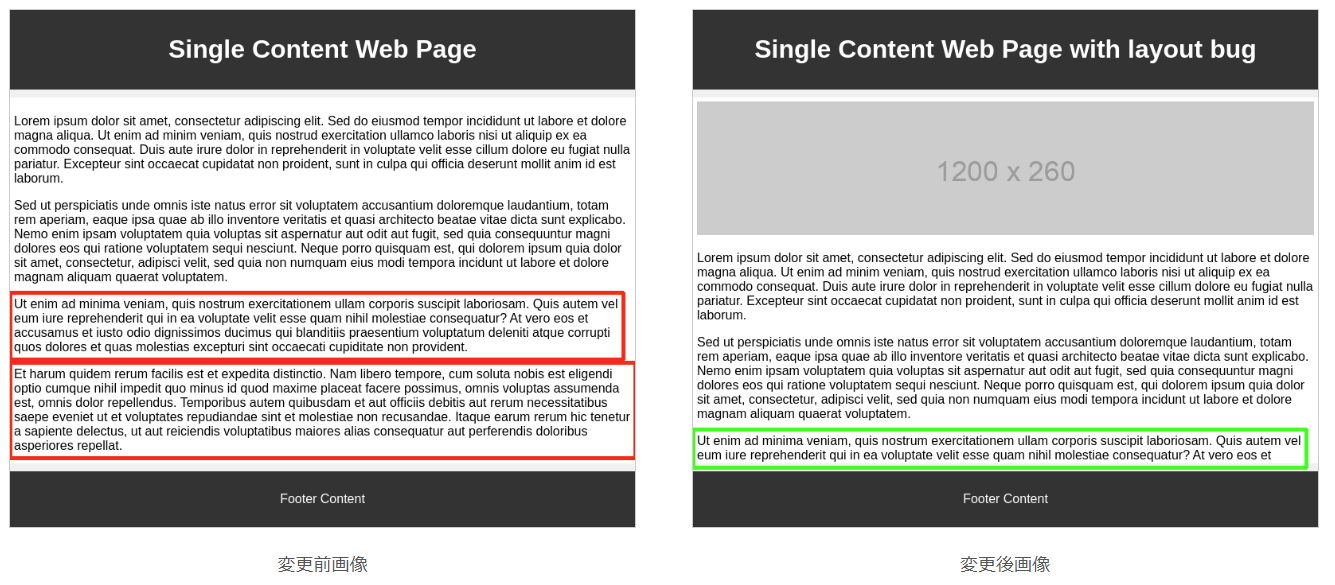
\includegraphics[width=1.0\columnwidth]{image/4_img_buf.png}
        \caption{「不具合箇所赤枠強調画像」と「不具合箇所緑枠強調画像」}
        \label{fig: img_bug}
    \end{center}
\end{figure}
\par
不具合抽出処理を、以下に示す。
\begin{enumerate}
    \item unique\_contours\_bfの各輪郭要素の数だけループして、以下の処理を行う。
          \begin{enumerate}
              \item unique\_contours\_afの各輪郭要素の数だけループして、以下の処理を行う。
                    \begin{enumerate}
                        % \item unique\_contours\_bfの輪郭に対するバウンディングボックスの座標とサイズを計算し、
                        %       そのバウンディングボックスに基づいてWebページの変更前画像から特定の領域を切り出す。
                        % \item unique\_contours\_afの輪郭に対するバウンディングボックスの座標とサイズを計算し、
                        %       そのバウンディングボックスに基づいてWebページの変更後画像から特定の領域を切り出す。
                        \item unique\_contours\_bfとunique\_contours\_afのそれぞれの輪郭要素のバウンディングボックスを、boundingRect関数を用いて取得する。
                        \item unique\_contours\_bfで取得したバウンディングボックスの座標とサイズに基づき、「変更前高解像度画像」から対応する画像領域region\_bfを抽出する。
                        \item unique\_contours\_afで取得したバウンディングボックスの座標とサイズに基づき、「変更後高解像度画像」から対応する画像領域region\_afを抽出する。
                        \item absdiff関数を用いて、region\_bfとregion\_afの画像領域間の各ピクセル値の絶対値の差を計算し、類似度を求める。
                        \item 類似度が9.5割を超えれば、レイアウトの不具合は無いと判定し、unique\_contours\_bfとunique\_contours\_afからそれぞれ現在処理中の輪郭要素を削除する。
                    \end{enumerate}
          \end{enumerate}
    \item boundingRect関数を用いて、unique\_contours\_bfとunique\_contours\_afのそれぞれの輪郭リストの各要素である輪郭データから、輪郭を囲む矩形の座標と幅、高さを取得する。
    \item 取得した矩形情報を引数に指定したrectangle関数を用いて、Webページの変更前画像上に赤枠、Webページの変更後画像上に緑枠を描画し、「不具合箇所赤枠強調画像」と「不具合箇所緑枠強調画像」を生成する。
\end{enumerate}


% \section{表示部}\label{sec:Interface_Display_Section}
% 表示部は、データ管理部によってdisp\_dirディレクトリ内に保存されたデータを受け取り、
% そのデータを、Flask\ref{sec:Flask}を用いて作成したローカルサーバ上のWebページに配置し、表示する。
% \toolName の実行コマンド初回実行時は、\ref{sec:Web_data_get_section}節で取得したWebページの画像を表示する。
% \toolName の実行コマンド2回目以降実行時は、初回実行時に取得する画像に加えて、\ref{sec:Difference_extraction_section}節で取得した画像、
% \ref{sec:Affected_area_extraction}節で生成した画像、\ref{sec:Layout_bug_extraction_section}節で生成した画像を表示する。
